\documentclass[12pt,english]{article}

\usepackage[utf8]{inputenc}
\usepackage{amsmath}
\usepackage{cite}
\usepackage{graphicx}
\usepackage[a4paper,bindingoffset=0.2in,left=1.25in,right=.75in,top=1in, bottom = 1in, footskip=.25in]{geometry}
\usepackage{fourier}
\usepackage{inconsolata}
\usepackage{minted}
\usepackage{nameref}
\usepackage{hyperref}

\renewcommand{\baselinestretch}{1.25}
\graphicspath{ {../images/} }
\usemintedstyle{tango}

\begin{document}
\begin{center}

\includegraphics[scale = 0.5]{LincolnLogo}
\newline\newline
\thispagestyle{empty}
    \textbf{\huge{Analysis of Shapes in Nature Using Advanced Mathematical and Computing Techniques} \\
    [100pt] \Large{Timothy Smith\\25796944} \\
    [40pt]\LARGE{Supervised by Dr Danilo Roccatano}\\
    [50pt]\today \\
	[40pt]Scientific Report in the 3\textsuperscript{rd} Year Module\\ MTH3009 Mathematics Project  }
\end{center}

\newpage
\section*{Abstract}
Placeholder abstract text

\newpage
\tableofcontents

\newpage
\section{Introduction}

\section{Theoretical Background}
\subsection{The Elliptic Fourier Transform}
The Fourier transform is a way of finding constituent frequencies within a function on the real domain.
The Fourier transform extends the concept of the Fourier series (which openerates on a bounded interval) to the real
domain.
That is to say, the Fourier Series operations on a periodic function with period
$P$ and decomposes it into a series of sinusoidal waves, while the Fourier transform
does the same but for any complex valued function $f(x)$.

[Get references from book from differential equations module]

The elliptic Fourier transform extends this concept to a finite series of points
on the $(x, y)$ plane. This is useful for practical applications in
computing because one of the most typical ways to model a two-dimensional curve in
a computer program is just that, a finite series of points on the $(x, y)$ plane.

The way that the elliptic Fourier transform works is by taking said
series of points and assuming that they are connected by straight lines, and modelling
$x$ and $y$ coordinates as periodic functions of a parameter $t$, such that
$x = x(t)$ and $y = y(t)$. Importantly, $x(t)$ and $y(t)$ have the same period $T$.

\subsubsection{The Fourier Series}
The Fourier series
(\ref{eq:fourierseries})
lets you take a single repeating unit of a
periodic function and use this to generate an infinite sum of
sinusoidal functions that converge to it.
This is useful because trigonmetric functions have mathematical
properties that not all functions posess, allowing you to work
with them nicely in more situations.
\begin{equation}
	\label{eq:fourierseries}
	s(x) \sim A_0 + \sum_{n=1}^{\infty} \left(
		A_n \cos \left( \frac{2\pi nx}{P} \right) +
		B_n \sin \left( \frac{2\pi nx}{P} \right)
	\right)
\end{equation}
The \(\sim\) symbol indicates that the series doesn't strictly
converge in all cases.

The coefficients \(A_0\), \(A_n\) and \(B_n\) are given by
(\ref{eq:fourierseriescoefficients}).

\begin{equation}
\label{eq:fourierseriescoefficients}
\begin{aligned}
	A_0 &= \frac{1}{P} \int_{-\frac{P}{2}}^{\frac{P}{2}}
		s(x) \,dx \\
	A_n &= \frac{1}{P} \int_{-\frac{P}{2}}^{\frac{P}{2}}
		s(x) \cos \left(\frac{2\pi nx}{P}\right) \,dx \\
	B_n &= \frac{1}{P} \int_{-\frac{P}{2}}^{\frac{P}{2}}
		s(x) \sin \left(\frac{2\pi nx}{P}\right) \,dx \\
\end{aligned}
\end{equation}

Here \(A_0\) is a constant, and \(A_n\) and \(B_n\) are functions of \(n\).
In fact, since both the denominator of the fraction and the range of the integral for \(A_0\) are the same, \(P\),
\(A_0\) is simply the average around which the function oscillates.

A good intuition for why the Fourier series works is that the
integral of the product of a function and a sinusoid is a measure
of how well that function \textit{matches} the sinusoid.
For example, the $\sin$ function perfectly matches itself since 
$\sin^2x$ has a positive average, while the $\sin$ and $\cos$
functions are a perfect anti-match since $\sin x \cos x$ simplifies
to $\frac{\sin 2x}{2}$ which averages around $0$.

\subsubsection{Exponential Form}
The concept of the Fourier series can actually be extended to the 
complex numbers $\mathbb{C}$.

This isn't terribly surprising, since there is a nice connection between the
complex numbers and trigonometric functions given by Euler's formula (\ref{eq:eulers}).
\begin{equation} \label{eq:eulers}
	e^{ix}=\cos{x}+i\sin{x}
\end{equation}
Thus if we take $A_n$  and $B_n$ from
(\ref{eq:fourierseriescoefficients})
we can let a new variable
\begin{displaymath}
	c_n = A_n + i B_n
\end{displaymath}
and we can get
\begin{equation}
	s(x) \sim A_0 + \sum_{n=1}^{\infty}
		c_ne^{i\frac{2\pi nx}{P}}
\end{equation}

\subsubsection{The Fourier Transform}
The transform function ($S(t)$) for frequency $f$ is given by
(\ref{fourier:transform}).
\begin{equation} \label{fourier:transform}
	S(t)=\int_{-\infty}^{\infty}s(t)\cdot \mathrm{e}^{-i2\pi ft} dt
\end{equation}

\subsubsection{Elliptical Fourier Analysis}
The seminal paper on this topic is \cite{kuhl:1982}.

For:
\begin{equation}
\begin{aligned}
	x(t) = A_0+\sum_{n=1}^{\infty}\left[a_n\cos\frac{2n\pi t}{T}+b_n\sin\frac{2n\pi t}{T}\right] \\
	y(t) = C_0+\sum_{n=1}^{\infty}\left[c_n\cos\frac{2n\pi t}{T}+d_n\sin\frac{2n\pi t}{T}\right]
\end{aligned}
\end{equation}

\be

This paper gives the coefficients (for a discrete set of points that form a closed contour):
\begin{equation}
\begin{aligned}
	a_n&=\frac{T}{2n^2\pi^2}\sum_{p=1}^{K}\left[\cos\frac{2n\pi t_p}{T}-\cos\frac{2n\pi t_{p-1}}{T}\right] \\
	b_n&=\frac{T}{2n^2\pi^2}\sum_{p=1}^{K}\left[\sin\frac{2n\pi t_p}{T}-\sin\frac{2n\pi t_{p-1}}{T}\right] \\
	c_n&=\frac{T}{2n^2\pi^2}\sum_{p=1}^{K}\left[\cos\frac{2n\pi t_p}{T}-\cos\frac{2n\pi t_{p-1}}{T}\right] \\
	d_n&=\frac{T}{2n^2\pi^2}\sum_{p=1}^{K}\left[\sin\frac{2n\pi t_p}{T}-\sin\frac{2n\pi t_{p-1}}{T}\right]
\end{aligned}
\end{equation}

It also gives the centres:

\begin{equation}
\begin{aligned}
	A_0 = \frac{1}{T}\sum_{p=1}^{K}\left[\frac{\Delta x_p}{2\Delta t_p}\left(t_p^2-t_{p-1}^2\right)+\xi_p\left(t_p-t_{p-1}\right) \right]\\
	C_0 = \frac{1}{T}\sum_{p=1}^{K}\left[\frac{\Delta y_p}{2\Delta t_p}\left(t_p^2-t_{p-1}^2\right)+\delta_p\left(t_p-t_{p-1}\right) \right]
\end{aligned}
\end{equation}

Where:

\begin{equation}
\begin{aligned}
	\xi_p = \sum_{j=1}^{p-1}\Delta x_j-\frac{\Delta x_p}{\Delta t_p}\sum_{j=1}^{p-1}\Delta t_j \\
	\delta_p = \sum_{j=1}^{p-1}\Delta y_j-\frac{\Delta y_p}{\Delta t_p}\sum_{j=1}^{p-1}\Delta t_j
\end{aligned}
\end{equation}

You can see this implemented in \nameref{code:grapharea}.

\subsection{Processing the Images}
In order to find shapes in our images for the purposes of analysis,
we will need to detect edges. For this we will use the Canny Edge
detection method, developed by John F. Canny.

\subsubsection{Convolution Kernels}
The most basic aspect of edge detection is the convolution kernel.
This is an $M{\times}M: \{M=2n+1, n\in\mathbb{N}\}$ matrix
(an odd sided square matrix).
Odd side lengths allow the kernel to be centered at each pixel.  If we let the function $f(x,y)$ represent the original image, $g(x,y)$ represent the convolved image and $\omega$
represent the kernel, then:
\begin{equation}
	g(x,y)=\sum_{i=-n}^{n}\sum_{j=-n}^{n}\omega(i,j)f(x-i,y-j)
\end{equation}
Notice that the coordinates of the kernel are not $1$ to $M$
as with a traditional matrix, but rather $-n$ to $n$.

The effect of this on an image will be to make each pixel of a
convolved image a function of the surrounding pixels.
The simplest convolution matrix is the identity convolution matrix,
(\ref{convm:identity}).
\begin{equation}
	\label{convm:identity}
	\begin{bmatrix}
		0 & 0 & 0\\
		0 & 1 & 0\\
		0 & 0 & 0\\
	\end{bmatrix}
\end{equation}
More examples include edge detection kernels like
(\ref{convm:edge1}) and (\ref{convm:edge2}).
\begin{center}
\begin{minipage}{.4\linewidth}
\begin{equation} \label{convm:edge1}
	\begin{bmatrix}
		 0 & -1 &  0\\
		-1 &  4 & -1\\
		 0 & -1 &  0\\
	\end{bmatrix}
\end{equation}
\end{minipage}
\begin{minipage}{.4\linewidth}
\begin{equation} \label{convm:edge2}
	\begin{bmatrix}
		-1 & -1 & -1\\
		-1 &  8 & -1\\
		-1 & -1 & -1\\
	\end{bmatrix}
\end{equation}
\end{minipage}
\end{center}

\subsubsection{Active Contours}

\subsubsection{Canny Edge Detection}

\pagebreak
\section{Results}
\subsection{Data Considered}
A set of images of leaves were taken from \cite[Fig. 111-8]{benson:1957}.

\begin{figure}[!hbt]
\begin{centre}
	\begin{minipage}{0.19\textwidth}
		\caption{Cordate}
		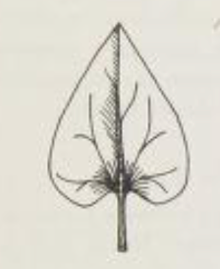
\includegraphics[width=\textwidth]{../code/contour/original/cordate}
	\end{minipage}
	\begin{minipage}{0.19\textwidth}
		\caption{Cuneate}
		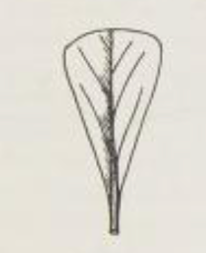
\includegraphics[width=\textwidth]{../code/contour/original/cuneate}
	\end{minipage}
	\begin{minipage}{0.19\textwidth}
		\caption{Deltoid}
		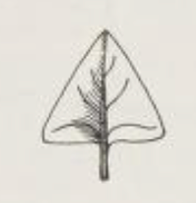
\includegraphics[width=\textwidth]{../code/contour/original/deltoid}
	\end{minipage}
	\begin{minipage}{0.19\textwidth}
		\caption{Elliptic}
		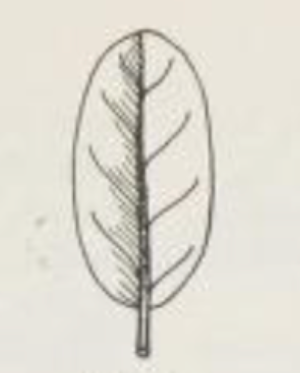
\includegraphics[width=\textwidth]{../code/contour/original/elliptic}
	\end{minipage}
	\begin{minipage}{0.19\textwidth}
		\caption{Hastate}
		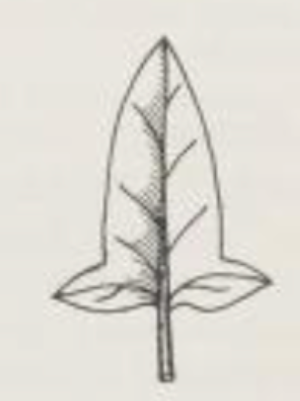
\includegraphics[width=\textwidth]{../code/contour/original/hastate}
	\end{minipage}
\end{centre}
\end{figure}

\begin{figure}[!hbt]
\begin{centre}
	\begin{minipage}{0.19\textwidth}
		\caption{Lanceolate}
		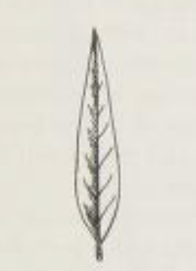
\includegraphics[width=\textwidth]{../code/contour/original/lanceolate}
	\end{minipage}
	\begin{minipage}{0.19\textwidth}
		\caption{Linear}
		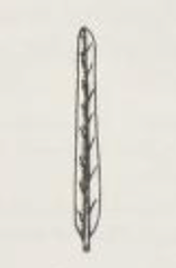
\includegraphics[width=\textwidth]{../code/contour/original/linear}
	\end{minipage}
	\begin{minipage}{0.19\textwidth}
		\caption{Obcordate}
		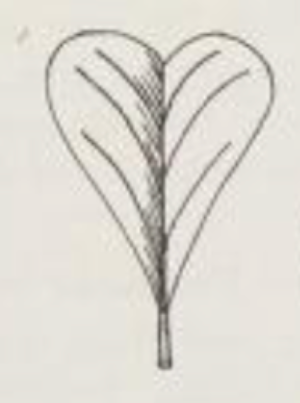
\includegraphics[width=\textwidth]{../code/contour/original/obcordate}
	\end{minipage}
	\begin{minipage}{0.19\textwidth}
		\caption{Obdeltoid}
		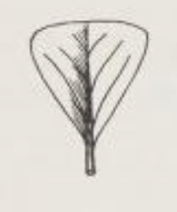
\includegraphics[width=\textwidth]{../code/contour/original/obdeltoid}
	\end{minipage}
	\begin{minipage}{0.19\textwidth}
		\caption{Oblanceolate}
		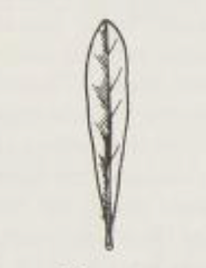
\includegraphics[width=\textwidth]{../code/contour/original/oblanceolate}
	\end{minipage}
\end{centre}
\end{figure}

\begin{figure}[!hbt]
\begin{centre}
	\begin{minipage}{0.19\textwidth}
		\caption{Oblong}
		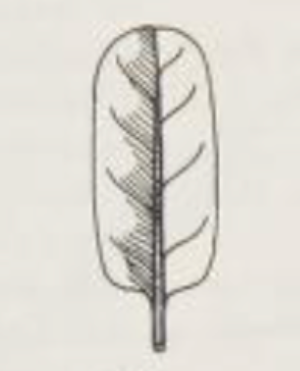
\includegraphics[width=\textwidth]{../code/contour/original/oblong}
	\end{minipage}
	\begin{minipage}{0.19\textwidth}
		\caption{Obovate}
		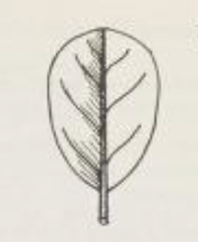
\includegraphics[width=\textwidth]{../code/contour/original/obovate}
	\end{minipage}
	\begin{minipage}{0.19\textwidth}
		\caption{Orbiculate}
		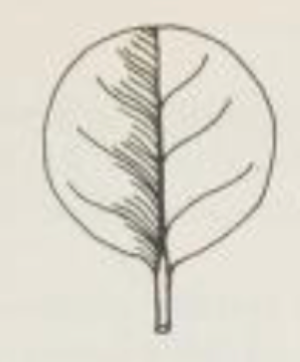
\includegraphics[width=\textwidth]{../code/contour/original/orbiculate}
	\end{minipage}
	\begin{minipage}{0.19\textwidth}
		\caption{Ovate}
		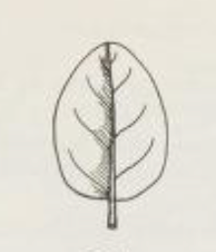
\includegraphics[width=\textwidth]{../code/contour/original/ovate}
	\end{minipage}
	\begin{minipage}{0.19\textwidth}
		\caption{Peltate}
		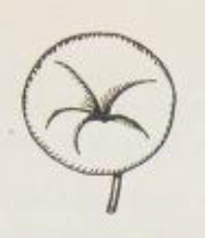
\includegraphics[width=\textwidth]{../code/contour/original/peltate}
	\end{minipage}
\end{centre}
\end{figure}

\begin{figure}[!hbt]
\begin{centre}
	\begin{minipage}{0.19\textwidth}
		\caption{Reniform}
		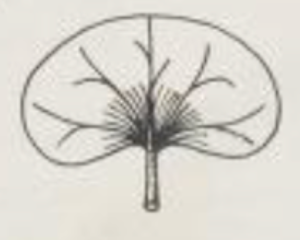
\includegraphics[width=\textwidth]{../code/contour/original/reniform}
	\end{minipage}
	\begin{minipage}{0.19\textwidth}
		\caption{Rhombic}
		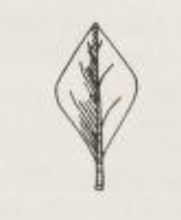
\includegraphics[width=\textwidth]{../code/contour/original/rhombic}
	\end{minipage}
	\begin{minipage}{0.19\textwidth}
		\caption{Sagitate}
		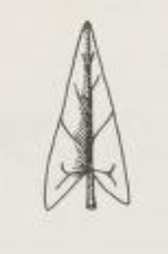
\includegraphics[width=\textwidth]{../code/contour/original/sagitate}
	\end{minipage}
	\begin{minipage}{0.19\textwidth}
		\caption{Spathulate}
		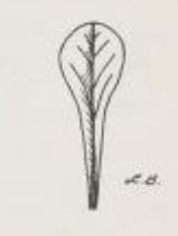
\includegraphics[width=\textwidth]{../code/contour/spathulate_with_signature}
	\end{minipage}
	\begin{minipage}{0.19\textwidth}
		\caption{Subulate}
		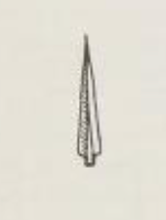
\includegraphics[width=\textwidth]{../code/contour/original/subulate}
	\end{minipage}
\end{centre}
\end{figure}
\pagebreak

\subsection{Image Processing}
These images were then processed using the MATLAB\textsuperscript{\textregistered} script \textbf{\nameref{code:contour}}
in order to produce comma--separated value (.csv) files with a series
of coordinates representing the contour.
This script is slightly inspired by work done previously in
the coursework for the \textit{Image Processing} module (\textbf{CMP3108}).

The images were first converted to grayscale and then black and white.
\begin{minted}{matlab}
    leaf_image = im2gray(leaf_image);
    leaf_image = imbinarize(leaf_image);
    ...
    leaf_image = 255 * leaf_image;
\end{minted}
As an example, figures (\ref{binarised:1}), (\ref{binarised:2}) and (\ref{binarised:3}) show what three of the leaf types looked like after
this process.
\begin{figure}[!hbt]
\begin{centre}
	\begin{minipage}{0.32\textwidth}
		\caption{Reniform (binarised)}
		\label{binarised:1}
		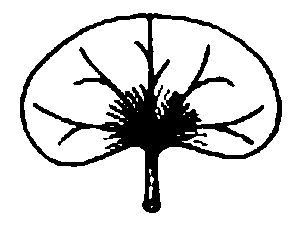
\includegraphics[width=\textwidth]{../code/contour/binarised/reniform}
	\end{minipage}
	\begin{minipage}{0.32\textwidth}
		\caption{Spathulate (binarised)}
		\label{binarised:2}
		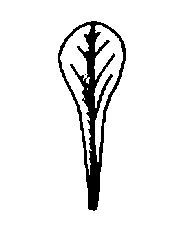
\includegraphics[width=\textwidth]{../code/contour/binarised/spathulate}
	\end{minipage}
	\begin{minipage}{0.32\textwidth}
		\caption{Subulate (binarised)}
		\label{binarised:3}
		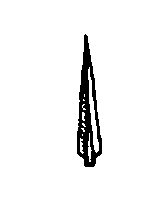
\includegraphics[width=\textwidth]{../code/contour/binarised/subulate}
	\end{minipage}
\end{centre}
\end{figure}

Next, an active contour was applied, creating a binary image deliniating the regions
for inside and outside the leaf.
\begin{minted}{matlab}
    leaf_contour = activecontour(leaf_image, contour_mask, 1000, "edge");
\end{minted}
Figures (\ref{contourmask:1}), (\ref{contourmask:2}) and (\ref{contourmask:3}) show what these three leaf types looked like after
this process.
\begin{figure}[!hbt]
\begin{centre}
	\begin{minipage}{0.32\textwidth}
		\caption{Reniform (after active contour)}
		\label{contourmask:1}
		
\includegraphics[width=\textwidth]{../code/contour/contour_mask/reniform}
	\end{minipage}
	\begin{minipage}{0.32\textwidth}
		\caption{Spathulate (after active contour)}
		\label{contourmask:2}
		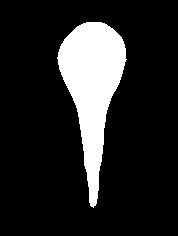
\includegraphics[width=\textwidth]{../code/contour/contour_mask/spathulate}
	\end{minipage}
	\begin{minipage}{0.32\textwidth}
		\caption{Subulate (after active contour)}
		\label{contourmask:3}
		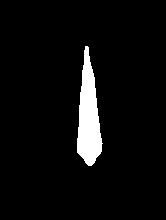
\includegraphics[width=\textwidth]{../code/contour/contour_mask/subulate}
	\end{minipage}
\end{centre}
\end{figure}

The final step is extracting a contour from these binary images
and write these contours to csv files.
This was done using MATLAB\textsuperscript{\textregistered}'s
built-in \verb|bwboundaries| function.
\begin{minted}{matlab}
    leaf_boundary = bwboundaries(leaf_contour, "noholes");
    ...
    leaf_boundary = leaf_boundary{1};
    writematrix(leaf_boundary, strcat("csv/", leaf_type, ".csv"));
\end{minted}

After this process is completed the code produces a graph of these
values for manual checking purposes.
\begin{minted}{matlab}
    plot(leaf_boundary(:,2), -leaf_boundary(:,1));
    axis equal;
\end{minted}
This actually proved invaluable since some of the images were initially broken,
with the contours containing unwanted invaginations. This turned out to be caused
by the initial boundary of the active contour being too thick and
encroaching on the leaves themselves. The solution was to lower the
thickness of the initial contour, by lowering the value of
\verb|contour_border_thickness| to 15 pixels.
\begin{minted}{matlab}
    contour_border_thickness = 15;
    contour_mask( ...
        contour_border_thickness:end-contour_border_thickness, ...
        contour_border_thickness:end-contour_border_thickness ...
    ) = 1;
\end{minted}
For examples of these graphs, see figures (\ref{contour:1}), (\ref{contour:2}) and (\ref{contour:3}).
\begin{figure}[!hbt]
\begin{centre}
	\begin{minipage}{0.32\textwidth}
		\caption{Reniform (contour graph)}
		\label{contour:1}
		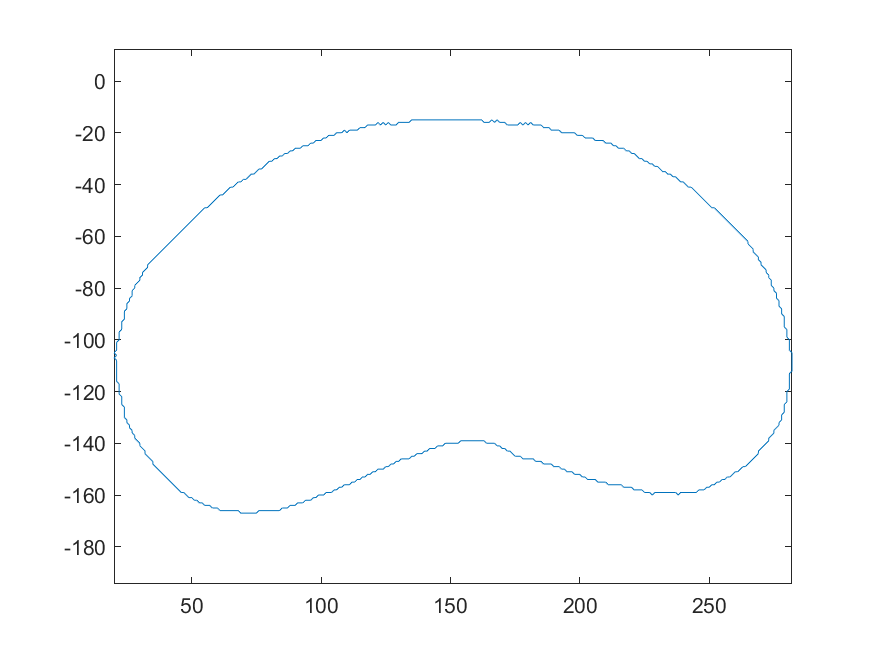
\includegraphics[width=\textwidth]{../code/contour/contour/reniform}
	\end{minipage}
	\begin{minipage}{0.32\textwidth}
		\caption{Spathulate (contour graph)}
		\label{contour:2}
		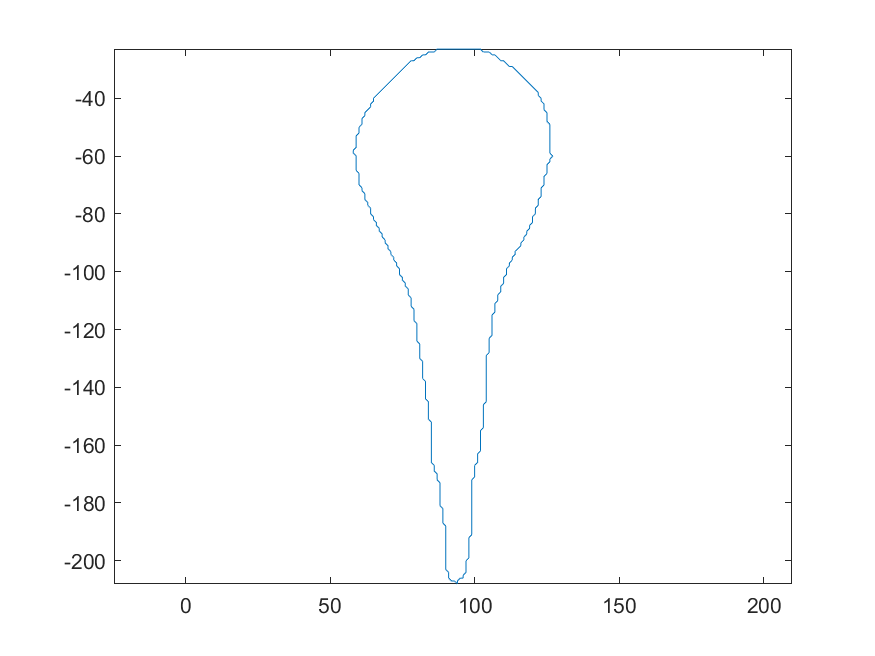
\includegraphics[width=\textwidth]{../code/contour/contour/spathulate}
	\end{minipage}
	\begin{minipage}{0.32\textwidth}
		\caption{Subulate (contour graph)}
		\label{contour:3}
		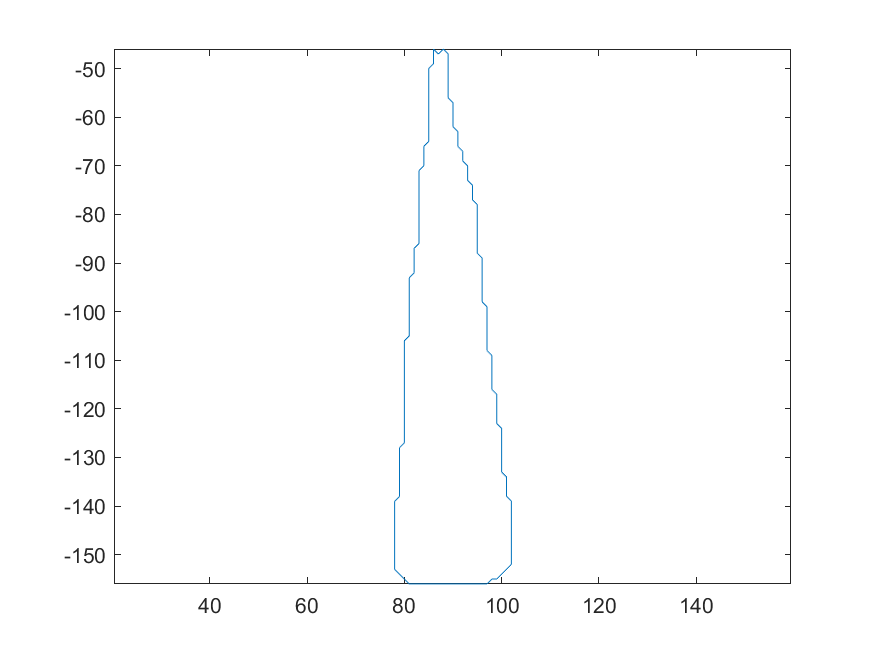
\includegraphics[width=\textwidth]{../code/contour/contour/subulate}
	\end{minipage}
\end{centre}
\end{figure}

\subsection{Elliptic Fourier Analysis}

\section{Conclusion}

\section{Acknowledgements}
I'd like to start by thanking paleontologists and science communicators
David Moscato and Will Harris of the \textit{Common Descent} podcast \cite{moscato:2024}
for sparking an interest in the life sciences that led me to choosing
this particular project subject.

I'd also like to thank my friends and family for supporting me throughout the project,
especially my friends Tom and Ruby for giving some much needed last-minute encouragement.

I'd also like to extend appreciation for my personal tutor, Bart Vorselaars,
for helping me with some personal issues in a way that took some stress off during
the later stages of this project.

Finally, and perhaps most importantly, I'd like to thank my project supervisor
Danilo Roccatano for assisting me effectively throughout the project and helping manage time
and prioritise tasks to meet the deadline near the end.

\pagebreak
\section{Bibliography}
\bibliographystyle{ieeetr}
\bibliography{refs}

\pagebreak
\section{Appendix}
All code used in this project can be found hosted on my personal GitHub
\cite{smith:2024}.

\subsection*{contour.m}
\label{code:contour}
\inputminted[breakanywhere=true, tabsize=4]{matlab}{../code/contour/contour.m}

\subsection*{graph\_area.cpp}
\label{code:grapharea}
\inputminted[breakanywhere=true, tabsize=4]{cpp}{../code/elliptic_fourier/graph_area.cpp}

\end{document}
